\section{Пример: данные о тестировании}
Давайте применим оценку стандартной ошибки по методу складного ножа к набору данных о результатах тестов $88$ студентов, приведенному в таблице 7.1. Напомним, что представляющая интерес статистика --- это отношение наибольшего собственного значения ковариационной матрицы к сумме собственных значений, как указано в (7.8)
\begin{equation}\label{eq11.12}
    \hat{\theta} = \hat{\lambda}_{1}/\sum\limits_{1}^{5}\hat{\lambda}_{i}.
\end{equation}
Чтобы применить метод складного ножа, мы удаляем по одному каждый случай (строку) в таблице 7.1 и вычисляем $\hat{\theta}$ для каждого набора данных размером $87$. На верхней части рисунка 11.1 показана гистограмма $88$ значений складного ножа $\hat{\theta}_{(i)}$.

Мы также вычислили $88$ бутстреп значений $\hat{\theta}$. Обратите внимание, что разброс гистограммы, полученной с помощью метода складного ножа, намного меньше, чем разброс бутстреп гистограммы, показанной на нижней части рисунка (мы принудительно задаем одну и ту же горизонтальную шкалу во всех гистограммах). Это иллюстрирует тот факт, что наборы данных складного ножа в среднем более похожи на исходный набор данных, чем бутстреп наборы данных. По средне на рисунке показана гистограмма <<завышенных>> значений складного ножа
\begin{equation}\label{eq11.13}
    \sqrt{87}(\hat{\theta}_{(i)} - \hat{\theta}_{(\cdot)})
\end{equation}
с разрывом в точке среднего складного ножа $\hat{\theta}_{(\cdot)}$. С этим коэффициентом увеличения гистограмма складного ножа похожа на бутсреп гистограмму, показанную на нижней части рисунка. Величина $\widehat{\text{se}}_{\text{jack}}$ оказывается равной $0.049$, что лишь немного больше, чем значение $0.047$ для бутстреп оценки, полученной в главе 7.

\noindent
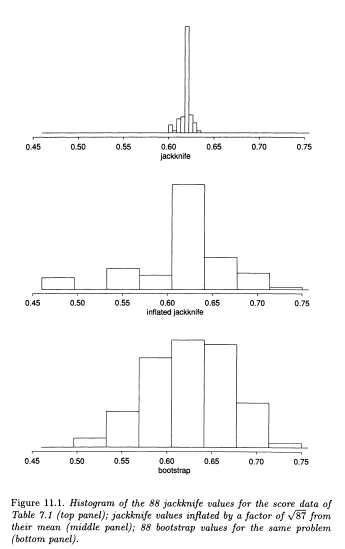
\includegraphics[width=\linewidth]{11/f11.1.png}
\newline